%%%%%%%%%%%%%%%%%%%%%%%%%%%%% Define Article %%%%%%%%%%%%%%%%%%%%%%%%%%%%%%%%%%
\documentclass[12pt]{article}
%%%%%%%%%%%%%%%%%%%%%%%%%%%%%%%%%%%%%%%%%%%%%%%%%%%%%%%%%%%%%%%%%%%%%%%%%%%%%%%

%%%%%%%%%%%%%%%%%%%%%%%%%%%%% Using Packages %%%%%%%%%%%%%%%%%%%%%%%%%%%%%%%%%%
\usepackage{geometry}
\usepackage{graphicx}
\usepackage{amssymb}
\usepackage{amsmath}
\usepackage{amsthm}
\usepackage{empheq}
\usepackage{mdframed}
\usepackage{booktabs}
\usepackage{lipsum}
\usepackage{color}
\usepackage{psfrag}
\usepackage{pgfplots}
\usepackage{bm}
\usepackage[export]{adjustbox}
\usepackage{float}
\usepackage{enumitem}
\usepackage{pythonhighlight}
\usepackage{tabularx}

%%%%%%%%%%%%%%%%%%%%%%%%%%%%%%%%%%%%%%%%%%%%%%%%%%%%%%%%%%%%%%%%%%%%%%%%%%%%%%%

% Other Settings

%%%%%%%%%%%%%%%%%%%%%%%%%% Page Setting %%%%%%%%%%%%%%%%%%%%%%%%%%%%%%%%%%%%%%%
\geometry{
  a4paper,
  total={170mm,257mm},
  left=0.75in,
  right=0.75in,
  top=0.75in,
  bottom=0.75in,
}

\setlist[itemize]{itemsep=-2pt}
\setlist[enumerate]{itemsep=-2pt}
\setlength{\parindent}{0px}

%%%%%%%%%%%%%%%%%%%%%%%%%% Define some useful colors %%%%%%%%%%%%%%%%%%%%%%%%%%
\definecolor{ocre}{RGB}{243,102,25}
\definecolor{mygray}{RGB}{243,243,244}
\definecolor{deepGreen}{RGB}{26,111,0}
\definecolor{shallowGreen}{RGB}{235,255,255}
\definecolor{deepBlue}{RGB}{61,124,222}
\definecolor{shallowBlue}{RGB}{235,249,255}
%%%%%%%%%%%%%%%%%%%%%%%%%%%%%%%%%%%%%%%%%%%%%%%%%%%%%%%%%%%%%%%%%%%%%%%%%%%%%%%

%%%%%%%%%%%%%%%%%%%%%%%%%% Define an orangebox command %%%%%%%%%%%%%%%%%%%%%%%%
\newcommand\orangebox[1]{\fcolorbox{ocre}{mygray}{\hspace{1em}#1\hspace{1em}}}
%%%%%%%%%%%%%%%%%%%%%%%%%%%%%%%%%%%%%%%%%%%%%%%%%%%%%%%%%%%%%%%%%%%%%%%%%%%%%%%

%%%%%%%%%%%%%%%%%%%%%%%%%%%% English Environments %%%%%%%%%%%%%%%%%%%%%%%%%%%%%
\newtheoremstyle{mytheoremstyle}{3pt}{3pt}{\normalfont}{0cm}{\rmfamily\bfseries}{}{1em}{{\color{black}\thmname{#1}~\thmnumber{#2}}\thmnote{\,--\,#3}}
\newtheoremstyle{myproblemstyle}{3pt}{3pt}{\normalfont}{0cm}{\rmfamily\bfseries}{}{1em}{{\color{black}\thmname{#1}~\thmnumber{#2}}\thmnote{\,--\,#3}}
\theoremstyle{mytheoremstyle}
\newmdtheoremenv[linewidth=1pt,backgroundcolor=shallowGreen,linecolor=deepGreen,leftmargin=0pt,innerleftmargin=20pt,innerrightmargin=20pt,]{theorem}{Theorem}[section]
\theoremstyle{mytheoremstyle}
\newmdtheoremenv[linewidth=1pt,backgroundcolor=shallowBlue,linecolor=deepBlue,leftmargin=0pt,innerleftmargin=20pt,innerrightmargin=20pt,]{definition}{Definition}[section]
\theoremstyle{myproblemstyle}
\newmdtheoremenv[linecolor=black,leftmargin=0pt,innerleftmargin=10pt,innerrightmargin=10pt,]{problem}{Problem}[section]
%%%%%%%%%%%%%%%%%%%%%%%%%%%%%%%%%%%%%%%%%%%%%%%%%%%%%%%%%%%%%%%%%%%%%%%%%%%%%%%

%%%%%%%%%%%%%%%%%%%%%%%%%%%%%%% Plotting Settings %%%%%%%%%%%%%%%%%%%%%%%%%%%%%
\usepgfplotslibrary{colorbrewer}
\pgfplotsset{width=8cm,compat=1.9}
%%%%%%%%%%%%%%%%%%%%%%%%%%%%%%%%%%%%%%%%%%%%%%%%%%%%%%%%%%%%%%%%%%%%%%%%%%%%%%%

%%%%%%%%%%%%%%%%%%%%%%%%%%%%%%% Title & Author %%%%%%%%%%%%%%%%%%%%%%%%%%%%%%%%
\title{Computer Vision}
\author{Laxman Desai}
%%%%%%%%%%%%%%%%%%%%%%%%%%%%%%%%%%%%%%%%%%%%%%%%%%%%%%%%%%%%%%%%%%%%%%%%%%%%%%%

\begin{document}

\maketitle
\tableofcontents

\pagebreak
\section{MNIST Classification}
  The MNIST (Modified National Institute of Standards and Technology) database is a large database of handwritten digits that is commonly used for training various image processing systems. It has a training set of 60,000 examples and a test set of 10,000 examples, and is a subset of a larger set available from NIST. The digits have been size-normalized and centered in a fixed-size image.
  
  We will attempt to train models to classify the dataset in this section.
  
  \subsection{Model Layers}
    Keras Layers are the functional building blocks of Keras Models. Each layer is fed with input information, they process this information, do some computation and hence produce the output. Further, this output of one layer is fed to another layer as its input.

    \begin{figure}[H]
      \centering
      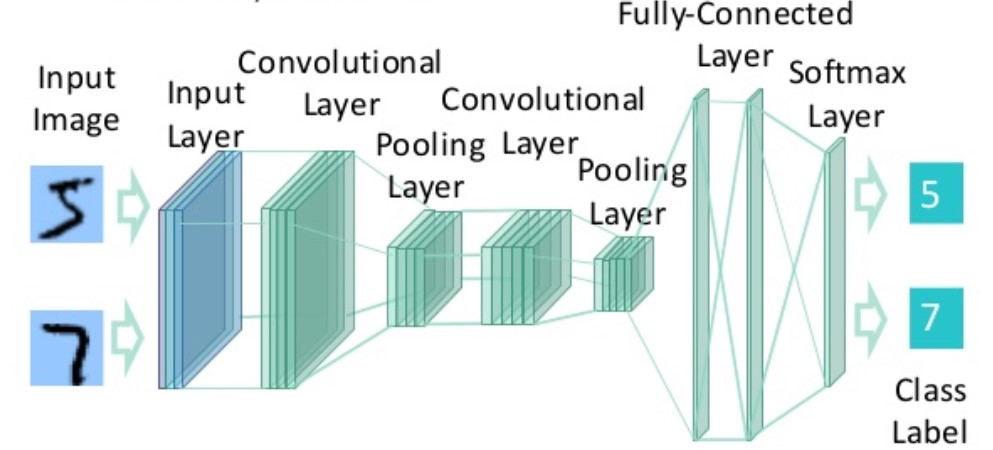
\includegraphics[width=0.75\textwidth]{images/layers.jpeg}
      \caption{Intuitive overview}
    \end{figure}

    \subsubsection{Input Layer}
    To understand the structure of the input data, Keras requires the shape of the input.The original input image is $28 \times 28$, so the \texttt{input\_shape = (28,28,1)}, where 1 indicates that number of color channels is 1.
  
    \subsubsection{Convolution Layer}
    This layer creates a convolution kernel. It is convolved over a single input to produce a tensor of outputs. If you are using this layer as the first layer of your model, provide \texttt{input\_shape} as the argument.
  
    \subsubsection{Max Pooling Layer}
    Maximum pooling is a pooling operation that calculates the largest value in each non overlapping patch of the feature map.
    
    The results are down sampled (or pooled feature) maps that highlight the most present feature in the patch. This method has been found to work better in practice than the average pooling method for computer vision tasks like image classification.
    
    Downsamples the input along its spatial dimensions (\texttt{height} and \texttt{width}) by taking the maximum value over an input window (of size defined by \texttt{pool\_size}) for each channel of the input. The window is shifted by \texttt{strides} along each dimension.

    \subsubsection{Flatten Layer}
    Flattens the the input.
    
    \begin{figure}[H]
      \centering
      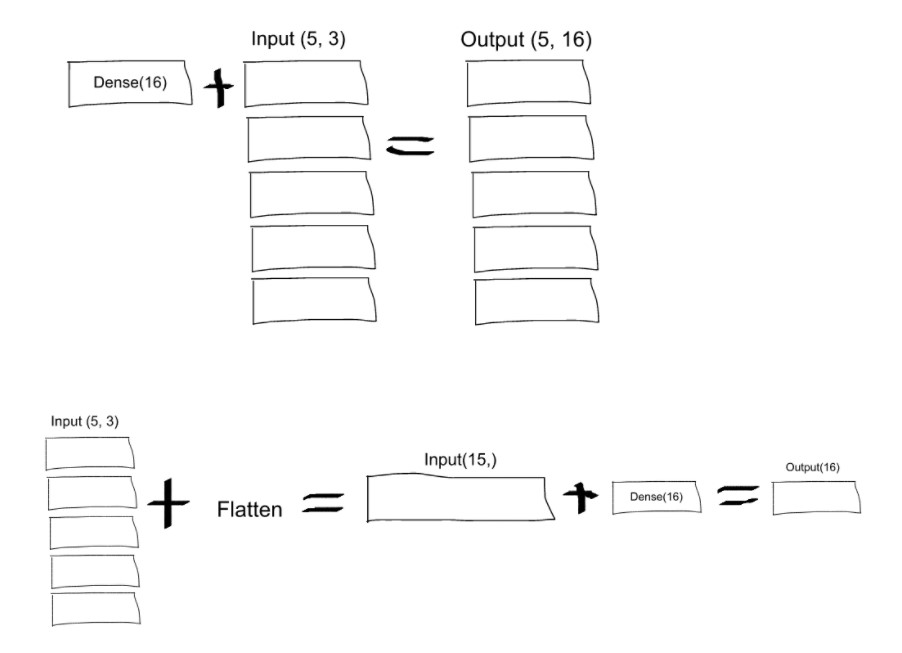
\includegraphics[width=0.75\textwidth]{images/flatten.jpg}
      \caption{Reason for the use of a flatten layer.}
    \end{figure}
    
    \subsubsection{Dropout Layer}
    You can implement dropout by added Dropout layers into our network architecture. The Dropout layer randomly sets input units to 0 with a given frequency. It prevents overfitting by helping you dropping-out user-defined hyperparameters. 

    \begin{figure}[H]
      \centering
      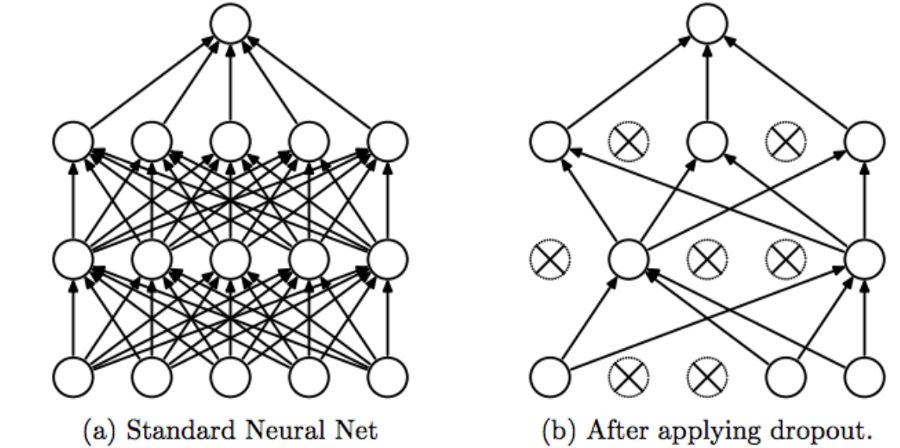
\includegraphics[width=0.75\textwidth]{images/dropout.png}
      \caption{Dropout in action. Crossed units on the right have been dropped.}
    \end{figure}

    \subsubsection{Softmax Dense Layer}
    The dense layer is one of the core layers. It is a standard neural network layer. It is helpful to produce output in the desired form.
    
  \subsection{Code}
  
    \subsubsection{Import modules:}
    \begin{python}
      import numpy as np
      from tensorflow import keras
      from tensorflow.keras import layers
    \end{python}

    \subsubsection{Load the dataset:}
    \begin{python}
      # Import the MNIST dataset
      from tensorflow.keras.datasets import mnist
      
      # Split data between training and testing sets
      (X_train, y_train), (X_test, y_test) = mnist.load_data()

      # Scale images from [0, 255] to the [0.0, 1.0] range
      X_train = X_train.astype('float32') / 255
      X_test = X_test.astype('float32') / 255

      # Add an extra dimention for the layers
      # Layers = 1 for grayscale images
      # Layers = 3 for RGB / HSV images

      X_train = np.expand_dims(X_train, -1)
      X_test = np.expand_dims(X_test, -1)
    \end{python}

    \subsubsection{Build the model:}
    \begin{python}
      model = keras.Sequential(
        [
          keras.Input(shape=input_shape),
          layers.Conv2D(32, kernel_size=(3, 3), activation="relu"),
          layers.MaxPooling2D(pool_size=(2, 2)),
          layers.Conv2D(64, kernel_size=(3, 3), activation="relu"),
          layers.MaxPooling2D(pool_size=(2, 2)),
          layers.Flatten(),
          layers.Dropout(0.5),
          layers.Dense(num_classes, activation="softmax"),
        ]
      )
      
      model.summary()
    \end{python}

    \newcolumntype{b}{X}
    \newcolumntype{s}{>{\hsize=.5\hsize}X}
    
    \hspace{-5px}\texttt{
    \begin{tabularx}{\textwidth}{b s s} 
      \hline
      Layer (type)                      &Output Shape             &Param \#     \\ [0.5ex] 
      \hline\hline
      conv2d (Conv2D)                   &(None, 26, 26, 32)       &320          \\
      max\_pooling2d (MaxPooling2D)     &(None, 13, 13, 32)       &0            \\
      conv2d\_1 (Conv2D)                &(None, 11, 11, 64)       &18496        \\
      max\_pooling2d\_1 (MaxPooling2D)  &(None, 5, 5, 64)         &0            \\
      flatten (Flatten)                 &(None, 1600)             &0            \\
      dropout (Dropout)                 &(None, 1600)             &0            \\
      dense (Dense)                     &(None, 10)               &16010        \\ [1ex]
      \hline
    \end{tabularx}
    }
    
    \vspace{10px}
    Total params: 34,826,
    Trainable params: 34,826,
    Non-trainable params: 0

    \subsubsection{Train the model:}
    \begin{python}
      batch_size = 128
      epochs = 15

      model.compile(loss="categorical_crossentropy", optimizer="adam",
        metrics=["accuracy"])

      model.fit(x_train, y_train, batch_size=batch_size, epochs=epochs,
        validation_split=0.1)
    \end{python}

\pagebreak
\section{Optical Character Recognition}

  We will try and build a model that can break CAPTCHAs. What's a CAPTCHA? It's basically a the test to determine if the user is a bot or a human. We will first attempt at breaking text based CAPTCHAs.
  
  \paragraph{Stages:}
  \begin{enumerate}
    \item Data acquisition
    \item Preprocessing
    \item Building a model
    \item Training the model
    \item Testing the model
  \end{enumerate}

  \subsection{Preprocessing}
    We cannot input an image directly for the OCR system. Some pre-processing has to be done on the image so that it becomes easy for the OCR model to recognize the information in the image.

    \paragraph{Preprocessing includes the following:}
    \begin{enumerate}
      \item Skew Correction
      \item Removing Lines (Horizontal \&  Vertical)
      \item Building a model
      \item Testing
    \end{enumerate}
    
    \subsubsection{Skew Correction}
      Image obtained from the previous stage may not be correctly oriented, It may be aligned at any angle. So we need to perform skew correction to make sure that the image forwarded to subsequent stages is correctly oriented.
      
      \begin{figure}[H]
        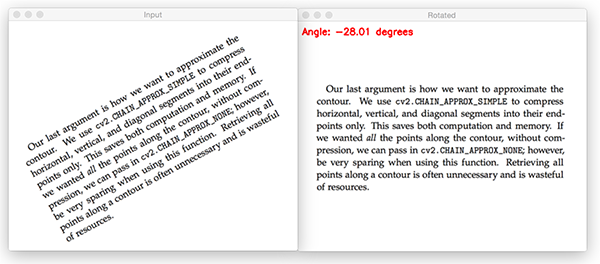
\includegraphics[width=0.75\textwidth, center]{images/2.png}
        \caption{Picture caption}
      \end{figure}
    
    \subsubsection{Binarization}
      That is, converting a coloured image to a black and white binary image. In practice, there exists an intermediate grayscale image.
      
      \begin{equation*}
        \text{Coloured image} \rightarrow \text{Grayscale image} \rightarrow \text{Binary image}
      \end{equation*}
      
      \begin{figure}[H]
        \centering
        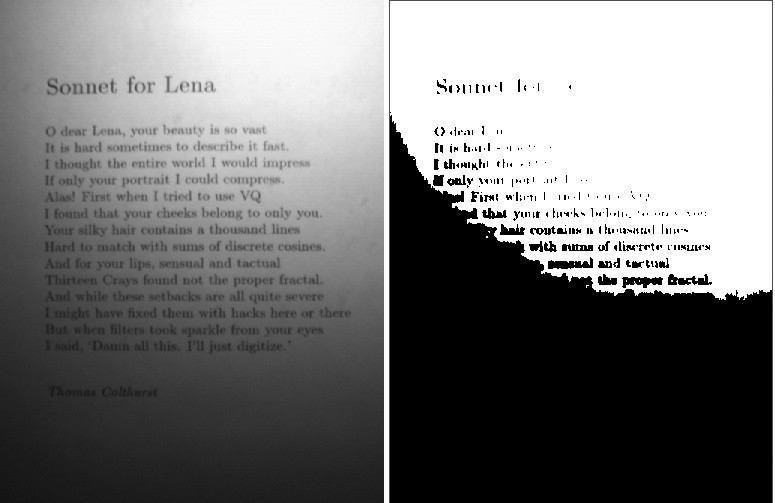
\includegraphics[width=0.75\textwidth]{images/1.jpeg}
        \caption{Binarization using a threshold on the image captured under non-uniform lighting.}
      \end{figure}

      Converting an RGB image to a grayscale image is easy. 
      To a computer, a black pixel has a value of 0 and a white pixel has a value of 255. Converting a grayscale to B\&W requires one to set a threshold value. If the pixel value is greater than the threshold, it is considered as a white pixel, else its as a black pixel. This naive strategy fails when lighting conditions are not uniform in the image. Here we can use Otsu's method or adaptive thresholding.
      
      \paragraph{Otsu's Binarization:}
      Since we are working with bimodal images, Otsu's algorithm tries to find a threshold value (t) which minimizes the weighted within-class variance given by the relation:
      
      \begin{equation*}
        \sigma_w^2(t) = q_1(t)\sigma_1^2(t)+q_2(t)\sigma_2^2(t)
      \end{equation*}
      
      where,
      
      \begin{align*}
        q_1(t) = \sum_{i=1}^{t} P(i) \quad &\& \quad q_2(t) = \sum_{i=t+1}^{I} P(i)
        \\
        \mu_1(t) = \sum_{i=1}^{t} \frac{iP(i)}{q_1(t)} \quad &\& \quad \mu_2(t) = \sum_{i=t+1}^{I} \frac{iP(i)}{q_2(t)}
        \\
        \sigma_1^2(t) = \sum_{i=1}^{t} [i-\mu_1(t)]^2 \frac{P(i)}{q_1(t)} \quad &\& \quad \sigma_2^2(t) = \sum_{i=t+1}^{I} [i-\mu_2(t)]^2 \frac{P(i)}{q_2(t)}
      \end{align*}
      
      \paragraph{Python code:} \
      \begin{python}
        import cv2 as cv

        # global thresholding
        ret1,th1 = cv.threshold(img,127,255,cv.THRESH_BINARY)

        # Otsu's thresholding
        ret2,th2 = cv.threshold(img,0,255,cv.THRESH_BINARY+cv.THRESH_OTSU)

        # Otsu's thresholding after Gaussian filtering
        blur = cv.GaussianBlur(img,(5,5),0)
        ret3,th3 = cv.threshold(blur,0,255,cv.THRESH_BINARY+cv.THRESH_OTSU)
      \end{python}
        
    % \subsubsection{Removing Lines (Horizontal \& Vertical)}
      

\end{document}